\documentclass[11pt]{article}

\usepackage[margin=1in]{geometry}
\usepackage{amsmath,amssymb,amsthm}
\usepackage{booktabs}
\usepackage{enumitem}
\usepackage{graphicx}
\usepackage{hyperref}
\usepackage{placeins}
\usepackage{xcolor}

\hypersetup{
  colorlinks=true,
  linkcolor=blue,
  citecolor=blue,
  urlcolor=blue
}

\newtheorem{definition}{Definition}
\newtheorem{remark}{Remark}

\newcommand{\R}{\mathbb{R}}
\newcommand{\Cov}{\operatorname{Cov}}
\newcommand{\spanop}{\operatorname{span}}

\title{A KRR Mechanism in In-Context Transformers\\
\large Condensed Lecture Notes}
\author{Fernando Ruiz Mazo}
\date{May 5, 2026}

\begin{document}

\maketitle

\section{The Question}

Pointwise agreement with KRR is weak: a transformer may satisfy \(F(y)\approx Ty\) at one label
vector without implementing the KRR label-response rule nearby. We therefore seek a layered
certificate.

\begin{enumerate}[label=\arabic*.]
\item \textbf{Fixed-geometry operator.} Freeze
\[
G=(X_{\mathrm{ctx}},X_{\mathrm{tgt}})
\]
and vary only \(y\). Then KRR is the linear operator \(T=K_tA^{-1}\).
\item \textbf{Behavior.} Test the local label response
\[
\text{does the transformer's local response }D_\varepsilon F(y)[u]\text{ match }Tu?
\]
on task-distributed directions \(u\sim\mathcal{N}(0,A)\), not arbitrary directions.
\item \textbf{Subspace sufficiency.} Can we extract from the context residual stream
\(H_\ell^{\mathrm{ctx}}\) a basis \(Q\) such that ridge still works when its dual search is
restricted to \(\spanop(Q)\)? With \(Q^\top A Q=I\), the restricted dual solution is
\(\alpha_Q(y)=QQ^\top y\). Since predictions are read through \(K_t\), the natural induced
operator is
\[
T_Q=K_tQQ^\top.
\]
Ask whether this restriction commits little prediction-relevant error, \(\rho_G(T_Q)\) small, and
whether the transformer's response follows it, \(E_\varepsilon(F,T_Q)\) small.
\item \textbf{Layerwise availability.} Compute the intrinsic prediction-risk rank \(r_T\) from the
finite KRR task, then ask where response spans \(C_\ell\) first contain a prefix
\(Q_{\ell,k}\) with \(k\approx r_T\) and \(\rho_G(T_{Q_{\ell,k}})\le0.05\).
\item \textbf{Causal use.} Remove high-task-leverage directions from \(Q\). A useful subspace should
be selective: keeping \(Q\) should preserve the task-local response, while removing important
\(Q\)-directions should damage it.
\end{enumerate}

The claim is local: in successful regimes, the transformer realizes the task-distributed KRR
label-response operator, explained by low-dimensional activation subspaces whose required dimension
is computed from the finite KRR task before seeing activations.

\section{Fixed Geometry Makes Ridge Regression an Operator}

Fix one episode:
\[
X_{\mathrm{ctx}}\in\R^{n_{\mathrm{ctx}}\times d_x},
\qquad
X_{\mathrm{tgt}}\in\R^{n_{\mathrm{tgt}}\times d_x}.
\]
The fixed geometry is
\[
G=(X_{\mathrm{ctx}},X_{\mathrm{tgt}}).
\]
During operator tests, only
\[
y=(y_1,\ldots,y_{n_{\mathrm{ctx}}})\in\R^{n_{\mathrm{ctx}}}
\]
varies. Define
\[
K=X_{\mathrm{ctx}}X_{\mathrm{ctx}}^\top,\qquad
K_t=X_{\mathrm{tgt}}X_{\mathrm{ctx}}^\top,\qquad
A=K+\sigma^2 I.
\]
Linear-kernel ridge regression gives
\[
\alpha^\star=A^{-1}y,\qquad
y^\star=K_t\alpha^\star=K_tA^{-1}y.
\]
Thus fixed-geometry ridge regression is the linear map
\[
T_G:=K_tA^{-1},
\qquad
T_G:\R^{n_{\mathrm{ctx}}}\to\R^{n_{\mathrm{tgt}}}.
\]
The transformer defines
\[
F_\theta^G:\R^{n_{\mathrm{ctx}}}\to\R^{n_{\mathrm{tgt}}},
\qquad
F_\theta^G(y)=\widehat y_\theta.
\]
When \(G\) is clear, write \(T\) and \(F\). The core test is not only \(F(y)\approx Ty\), but
whether the local label-response operator of \(F\) matches \(T\).

\section{Context-Label Directions, Local Operators, and Additivity}

A context-label direction is
\[
u\in\R^{n_{\mathrm{ctx}}},
\]
and perturbing labels in direction \(u\) means
\[
y+\varepsilon u
=
(y_1+\varepsilon u_1,\ldots,y_{n_{\mathrm{ctx}}}+\varepsilon u_{n_{\mathrm{ctx}}}).
\]
Pointwise agreement checks
\[
F(y)\approx Ty.
\]
Since ridge is linear,
\[
J_T(y)=T\quad\text{for every }y.
\]
The local version of ``same label-to-prediction rule'' is
\[
J_F(y)u\approx Tu,
\]
or, for small \(\delta\),
\[
F(y+\delta)\approx F(y)+T\delta.
\]
Estimate the Jacobian action by the central finite difference
\[
D_\varepsilon F(y)[u]
:=
\frac{F(y+\varepsilon u)-F(y-\varepsilon u)}{2\varepsilon}.
\]
The behavioral operator test is
\[
D_\varepsilon F(y)[u]\approx Tu.
\]
This is tangent-level agreement only. Matching value and derivative at one point does not imply
global equality.

The main probe law is task-label:
\[
u\sim\mathcal{N}(0,A).
\]
Indeed, under the matched linear task
\[
y=X_{\mathrm{ctx}}\beta+\eta,\qquad
\beta\sim\mathcal{N}(0,I),\qquad
\eta\sim\mathcal{N}(0,\sigma^2I),
\]
conditioning on \(G\) gives
\[
y\mid G\sim\mathcal{N}(0,X_{\mathrm{ctx}}X_{\mathrm{ctx}}^\top+\sigma^2I)
=\mathcal{N}(0,A),
\]
so
\[
\Cov(y\mid G)=A.
\]
Equivalently,
\[
u=A^{1/2}z,\qquad z\sim\mathcal{N}(0,I).
\]
The isotropic comparison law is
\[
u\sim\mathcal{N}(0,I).
\]
The claim is task-local because task probes are emphasized by the data-generating distribution;
isotropic probes test arbitrary context-label directions.

For held-out probes \(U=\{u_1,\ldots,u_m\}\) and a fixed linear operator
\(S:\R^{n_{\mathrm{ctx}}}\to\R^{n_{\mathrm{tgt}}}\), define
\[
E_\varepsilon(F,S;U)
:=
\left(
\frac{
\sum_{j=1}^m\|D_\varepsilon F(y)[u_j]-Su_j\|_2^2
}{
\sum_{j=1}^m\|Tu_j\|_2^2+\eta_{\mathrm{num}}
}
\right)^{1/2}.
\]
When \(S=T\), this measures local KRR response error, normalized by KRR response energy.

Ridge is additive:
\[
T(u+v)=Tu+Tv.
\]
A nonlinear \(F\) need not satisfy
\[
D_\varepsilon F(y)[u+v]\approx D_\varepsilon F(y)[u]+D_\varepsilon F(y)[v].
\]
For paired directions \(V=\{(u_j,v_j)\}_{j=1}^m\), define
\[
C_j =
F(y+\varepsilon u_j+\varepsilon v_j)
-F(y+\varepsilon u_j-\varepsilon v_j)
-F(y-\varepsilon u_j+\varepsilon v_j)
+F(y-\varepsilon u_j-\varepsilon v_j),
\]
and
\[
A_\varepsilon(F;V)
:=
\left(
\frac{
\sum_{j=1}^m\|C_j\|_2^2
}{
\sum_{j=1}^m\|T(\varepsilon u_j+\varepsilon v_j)\|_2^2+\eta_{\mathrm{num}}
}
\right)^{1/2}.
\]
For any affine label map, \(C_j=0\). This diagnostic checks whether a local linear operator
comparison is meaningful at the chosen \(\varepsilon\) and probe law.

\section{Activation Subspaces and Prediction-Risk Rank}

Behavioral certificates are
\[
F(y)\approx Ty,\qquad D_\varepsilon F(y)[u]\approx Tu.
\]
The subspace question is: can we extract from the context residual stream a basis \(Q\) such that,
if the KRR dual solution is forced to lie in \(\spanop(Q)\), the induced predictor still behaves
like full KRR in prediction-relevant directions? This makes the reduced operator a constrained KRR
object, not an arbitrary fitted readout.

Ridge uses context-position dual variables:
\[
\alpha^\star(y)=A^{-1}y\in\R^{n_{\mathrm{ctx}}},
\qquad
Ty=K_t\alpha^\star(y).
\]
At layer \(\ell\), the context residual stream is
\[
H_\ell^{\mathrm{ctx}}\in\R^{n_{\mathrm{ctx}}\times D}.
\]
Each column \(H_\ell^{\mathrm{ctx}}[:,k]\) is a context-position pattern in
\(\R^{n_{\mathrm{ctx}}}\). Hence linear combinations of residual-stream columns can define
candidate subspaces for the dual variable \(\alpha\).

Let
\[
Q=[q_1,\ldots,q_r]\in\R^{n_{\mathrm{ctx}}\times r},
\qquad
\spanop(Q)=\{Qc:c\in\R^r\}\subseteq\R^{n_{\mathrm{ctx}}}.
\]
Use an \(A\)-orthonormal basis:
\[
Q^\top A Q=I.
\]
This is the ridge dual geometry, since the quadratic energy is \(\frac12\alpha^\top A\alpha\).

Full ridge solves
\[
\alpha^\star(y)
=
\arg\min_{\alpha\in\R^{n_{\mathrm{ctx}}}}
\left\{
\frac12\alpha^\top A\alpha-\alpha^\top y
\right\},
\]
whose first-order condition gives \(\alpha^\star=A^{-1}y\). Restrict to
\(\alpha=Qc\):
\[
\frac12 c^\top Q^\top A Qc-c^\top Q^\top y
=
\frac12 c^\top c-c^\top Q^\top y.
\]
Then
\[
c^\star=Q^\top y,
\qquad
\alpha_Q(y)=QQ^\top y.
\]
Without \(A\)-orthonormality,
\[
\alpha_Q(y)=Q(Q^\top A Q)^{-1}Q^\top y.
\]
Predictions use \(K_t\), so once the restricted dual solution is \(\alpha_Q(y)=QQ^\top y\), the
corresponding induced operator is forced to be
\[
T_Q:=K_tQQ^\top.
\]
This is natural because it is exactly the full KRR prediction rule \(K_t\alpha\), with only the
allowed dual search space changed. It is not a free probe: the readout is KRR-constrained.

Prediction relevance is task-weighted. Conditional on \(G\),
\[
y\mid G\sim\mathcal{N}(0,A),
\qquad
u\sim\mathcal{N}(0,A).
\]
The reference target is the latent noise-free vector
\[
f_{\mathrm{tgt}}
=
\bigl(f(x^{\mathrm{tgt}}_1),\ldots,f(x^{\mathrm{tgt}}_{n_{\mathrm{tgt}}})\bigr)
\in\R^{n_{\mathrm{tgt}}},
\]
with \(K_{tt}=X_{\mathrm{tgt}}X_{\mathrm{tgt}}^\top\) in the linear case. Under the matched GP/KRR
model,
\[
\begin{bmatrix}
y\\
f_{\mathrm{tgt}}
\end{bmatrix}
\Bigm|G
\sim
\mathcal{N}\!\left(
0,
\begin{bmatrix}
A & K_t^\top\\
K_t & K_{tt}
\end{bmatrix}
\right).
\]
Gaussian conditioning gives
\[
\mathbb{E}[f_{\mathrm{tgt}}\mid y,G]=K_tA^{-1}y=Ty
\]
and
\[
\operatorname{Cov}(f_{\mathrm{tgt}}\mid y,G)
=
K_{tt}-K_tA^{-1}K_t^\top .
\]
We need a scale for approximation error. Exact KRR is the posterior mean, but it is not perfect:
even after observing \(y\), the latent target values still have posterior uncertainty. That
unavoidable uncertainty is the irreducible KRR posterior prediction risk:
\[
R_{\mathrm{KRR}}(G)
:=
\mathbb{E}\|f_{\mathrm{tgt}}-Ty\|_2^2
=
\operatorname{tr}\!\left(K_{tt}-K_tA^{-1}K_t^\top\right).
\]

For any linear approximation \(S\), decompose
\[
f_{\mathrm{tgt}}-Sy
=
\bigl(f_{\mathrm{tgt}}-Ty\bigr)
+
\bigl(T-S\bigr)y.
\]
The posterior residual is orthogonal to every function of \(y\). Indeed,
\[
\mathbb{E}\!\left[f_{\mathrm{tgt}}-Ty\mid y,G\right]
=
\mathbb{E}[f_{\mathrm{tgt}}\mid y,G]-Ty
=0,
\]
so for any measurable \(g(y)\),
\[
\mathbb{E}\left[\langle f_{\mathrm{tgt}}-Ty,g(y)\rangle\mid G\right]
=
\mathbb{E}\left[
\left\langle
\mathbb{E}[f_{\mathrm{tgt}}-Ty\mid y,G],g(y)
\right\rangle
\mid G
\right]
=0.
\]
Taking \(g(y)=(T-S)y\) kills the cross-term, hence
\[
\mathbb{E}\|f_{\mathrm{tgt}}-Sy\|_2^2
=
R_{\mathrm{KRR}}(G)
+
\mathbb{E}_{y\sim\mathcal{N}(0,A)}\|(T-S)y\|_2^2.
\]
Define the excess-risk ratio
\[
\rho_G(S)
:=
\frac{
\mathbb{E}_{y\sim\mathcal{N}(0,A)}\|(T-S)y\|_2^2
}{
R_{\mathrm{KRR}}(G)+\eta_{\mathrm{num}}
}.
\]
Here \(S\) is any candidate label-to-target linear operator: it may be an arbitrary low-rank
approximation, or later the activation-constrained operator \(T_Q\). The ratio says exactly how much
posterior prediction risk is added by replacing exact KRR \(T\) with \(S\):
\[
\mathbb{E}\|f_{\mathrm{tgt}}-Sy\|_2^2
=
R_{\mathrm{KRR}}(G)
+\rho_G(S)\bigl(R_{\mathrm{KRR}}(G)+\eta_{\mathrm{num}}\bigr).
\]
Ignoring the tiny numerical stabilizer, \(\rho_G(S)=0.05\) means ``five percent above KRR risk''.

The prediction-risk rank asks a different, intrinsic question: if we are allowed to choose the best
rank-\(r\) linear replacement for \(T\), how large must \(r\) be before \(\rho_G(S)\) is at most the
chosen tolerance? To answer this, rewrite the same excess-risk term in whitened task-label
coordinates.

Whiten task-label directions:
\[
y=A^{1/2}z,\qquad z\sim\mathcal{N}(0,I).
\]
Then
\[
Ty=K_tA^{-1}A^{1/2}z
=K_tA^{-1/2}z.
\]
Define the whitened KRR response operator
\[
C_G:=K_tA^{-1/2}.
\]
For any candidate \(S\), define its whitened response
\[
B_S:=SA^{1/2}.
\]
Then
\[
\mathbb{E}_{y\sim\mathcal{N}(0,A)}\|(T-S)y\|_2^2
=
\mathbb{E}_{z\sim\mathcal{N}(0,I)}\|(C_G-B_S)z\|_2^2
=
\|C_G-B_S\|_F^2.
\]
\textbf{This is the important coordinate change.} The approximation error is not
\(\|C_G-S\|_F^2\). The operator \(S\) acts on unwhitened labels \(y\), while \(C_G\) acts on
whitened coordinates \(z\). Therefore \(S\) must be moved into the same whitened coordinates before
comparison:
\[
S\quad\longmapsto\quad B_S=SA^{1/2}.
\]
Thus \(S\) has not disappeared; it appears as \(SA^{1/2}\). The rank problem is the problem of
approximating \(C_G\) by \(B_S=SA^{1/2}\), and then mapping back to label coordinates by
\(S=B_SA^{-1/2}\).

Let
\[
C_G=U\operatorname{diag}(s_i)V^\top,
\qquad
s_1\ge s_2\ge\cdots\ge0.
\]
Since \(z\) is isotropic,
\[
\mathbb{E}\|C_Gz\|_2^2=\sum_i s_i^2.
\]
By Eckart--Young, the best rank-\(r\) whitened response keeps the first \(r\) singular modes. Write
\[
C_{G,r}:=U_{:,1:r}\operatorname{diag}(s_1,\ldots,s_r)V_{:,1:r}^\top,
\qquad
S_r:=C_{G,r}A^{-1/2}.
\]
Then \(S_r\) is the best rank-\(r\) label-to-target operator for the task-weighted excess-risk
metric. It is chosen precisely so that its whitened version is the truncated KRR response:
\[
S_rA^{1/2}=C_{G,r}.
\]
Therefore it leaves
\[
\sum_{i>r}s_i^2.
\]
\textbf{The tail is not the risk of \(C_G\) by itself.} It is the excess-risk term for the
particular oracle choice \(S=S_r\):
\[
\mathbb{E}_{y\sim\mathcal{N}(0,A)}\|(T-S_r)y\|_2^2
=
\|C_G-S_rA^{1/2}\|_F^2
=
\|C_G-C_{G,r}\|_F^2
=
\sum_{i>r}s_i^2.
\]
Its total prediction risk is
\[
R_{\mathrm{KRR}}(G)+\sum_{i>r}s_i^2.
\]

\begin{definition}[Prediction-risk rank]
For fixed geometry \(G\) and tolerance \(\alpha>0\), define
\[
r_\alpha(G)
:=
\min\left\{
r:
\sum_{i>r}s_i^2
\le
\alpha R_{\mathrm{KRR}}(G)
\right\}.
\]
\end{definition}

In the experiments,
\[
r_T:=r_{5\%},
\]
so \(r_T\) is the smallest rank whose best reduced KRR response has prediction risk at most five
percent above exact KRR:
\[
\mathbb{E}\|f_{\mathrm{tgt}}-S_r y\|_2^2
\le
1.05\,\mathbb{E}\|f_{\mathrm{tgt}}-Ty\|_2^2
=
1.05\,R_{\mathrm{KRR}}(G),
\]
where \(S_r\) is the optimal rank-\(r\) reduced KRR response in whitened task-label coordinates.
With \(\eta_{\mathrm{num}}=0\), the same statement for any reduced operator \(S\) is
\[
\rho_G(S)\le0.05
\quad\Longleftrightarrow\quad
\mathbb{E}\|f_{\mathrm{tgt}}-Sy\|_2^2
\le
1.05\,\mathbb{E}\|f_{\mathrm{tgt}}-Ty\|_2^2.
\]
With the stabilizer present, this equivalence is understood up to the negligible
\(\eta_{\mathrm{num}}\) correction.
This is not the algebraic rank of \(T\). It is the number of task-visible KRR modes needed for
prediction equivalence at the chosen tolerance. A particular activation subspace \(Q\) of dimension
\(r_T\) still has to align with those modes; success requires \(\rho_G(T_Q)\le0.05\).

The activation-subspace test is therefore representation-dependent. The intrinsic rank \(r_T\)
uses the oracle operator \(S_r\), which is built directly from the singular modes of \(C_G\). The
actual certificate uses \(S=T_Q\), where \(Q\) is extracted from hidden states and the readout is
forced to be the KRR readout \(K_tQ\). Equal dimension alone does not imply equal risk.

For an activation basis \(Q\), set
\[
C_G=K_tA^{-1/2},\qquad W=A^{1/2}Q,\qquad P_Q=WW^\top .
\]
For \(u=A^{1/2}z\),
\[
Tu=C_Gz,\qquad
T_Qu=K_tQQ^\top A^{1/2}z=C_GP_Qz.
\]
Thus
\[
\rho_G(T_Q)
=
\frac{\|C_G(I-P_Q)\|_F^2}{R_{\mathrm{KRR}}(G)+\eta_{\mathrm{num}}}.
\]
If \(W\) spans the top \(r\) right singular directions of \(C_G\), then
\[
\rho_G(T_Q)
=
\frac{\sum_{i>r}s_i^2}{R_{\mathrm{KRR}}(G)+\eta_{\mathrm{num}}}.
\]
Hence \(\dim\spanop(Q)\ge r_T\) is necessary but not sufficient; alignment with leading
task-label modes is also required.

\begin{remark}[Reading the numbers]
\(\rho_G(S)=0.05\) means that using \(S\) instead of exact KRR adds five percent of the KRR
posterior prediction risk. The finite-difference errors \(E_\varepsilon(F,T)\) and
\(E_\varepsilon(F,T_Q)\) are separate operator-response diagnostics.
\end{remark}

The mechanism checks are
\[
E_\varepsilon(F,T;U)\ \text{small},
\qquad
\rho_G(T_Q)\ \text{small},
\qquad
E_\varepsilon(F,T_Q;U)\ \text{small}.
\]
The decomposition
\[
D_\varepsilon F(y)[u]-Tu
=
\bigl(D_\varepsilon F(y)[u]-T_Qu\bigr)
+
\bigl(T_Qu-Tu\bigr)
\]
separates model-subspace mismatch from reduced-KRR approximation error.

To extract an \(A\)-orthonormal subspace from any context-pattern matrix
\(M\in\R^{n_{\mathrm{ctx}}\times p}\), compute
\[
A^{1/2}M=U\Sigma V^\top,
\]
keep selected left singular directions, and map back:
\[
Q(M):=A^{-1/2}U_{\mathrm{kept}}.
\]
Then \(Q(M)^\top A Q(M)=I\). The raw final-state extractor is
\[
M_{\mathrm{raw}}=H_L^{\mathrm{ctx}},
\qquad
Q_{\mathrm{raw}}:=Q(M_{\mathrm{raw}}).
\]
The response-only extractor uses
\[
Z_L(u)=
\frac{
H_L^{\mathrm{ctx}}(y+\varepsilon u)-H_L^{\mathrm{ctx}}(y-\varepsilon u)
}{2\varepsilon},
\qquad
M_{\mathrm{resp}}=[Z_L(u_1),\ldots,Z_L(u_m)],
\]
and
\[
Q_{\mathrm{resp}}:=Q(M_{\mathrm{resp}}).
\]
After extraction, \(Q\) is frozen. The certificate is a fixed activation-derived \(T_Q\) that is
prediction-risk sufficient and matches held-out local responses.

\section{Layerwise Availability Construction}

The layerwise diagnostic asks when a KRR-sufficient response subspace becomes available. At layer
\(\ell\),
\[
Z_\ell(u)
:=
\frac{
H_\ell^{\mathrm{ctx}}(y+\varepsilon u)-H_\ell^{\mathrm{ctx}}(y-\varepsilon u)
}{2\varepsilon}.
\]
Stack build probes:
\[
M_\ell=[Z_\ell(u_1),\ldots,Z_\ell(u_m)].
\]
An \(A\)-weighted SVD gives
\[
A^{1/2}M_\ell=U_\ell\Sigma_\ell V_\ell^\top,
\qquad
q_i=A^{-1/2}U_{\ell,i}.
\]
Write the singular values as
\[
\sigma_{\ell,1}\ge\sigma_{\ell,2}\ge\cdots.
\]
There are two separate steps. Conceptually, we can keep all singular directions of
\(A^{1/2}M_\ell\) and test all prefixes. In exact arithmetic this means keeping all directions with
\(\sigma_{\ell,i}>0\). In finite precision, near-zero singular directions are unstable and mostly
encode numerical noise, so the implementation uses only a mild numerical guard:
\[
d_\ell
=
\min\left\{
r_{\max},
\#\{i:\sigma_{\ell,i}\ge\tau_{\mathrm{sv}}\sigma_{\ell,1}\}
\right\},
\]
with \(r_{\max}\) the candidate-rank cap. Taking \(\tau_{\mathrm{sv}}=0\) would correspond to trying
all nonzero directions. Then the activation-derived candidate response span is
\[
C_\ell
=
[q_1,\ldots,q_{d_\ell}],
\qquad
C_\ell^\top A C_\ell=I.
\]
Thus \(C_\ell\) is the context-position span made visible by label motion at layer \(\ell\), up to
finite-precision cleanup. This truncation is not the KRR sufficiency criterion; it only prevents
near-null numerical directions from entering the candidate activation span.

The principled step comes next. Inside \(C_\ell\), order directions by KRR usefulness. If
\(C_\ell\) is \(A\)-orthonormal, set
\[
W_\ell=A^{1/2}C_\ell,
\qquad
Z=K_tA^{-1/2}.
\]
The eigenvectors of
\[
W_\ell^\top Z^\top ZW_\ell
\]
ordered from largest to smallest define nested prefixes
\[
Q_{\ell,0}\subset Q_{\ell,1}\subset\cdots\subset C_\ell.
\]
This produces the best KRR-aligned prefixes available inside the activation-derived span. It is an
availability test, not a claim about the transformer's internal basis choice. For each prefix,
\[
T_{Q_{\ell,k}}=K_tQ_{\ell,k}Q_{\ell,k}^\top
\]
and
\[
\rho_G(T_{Q_{\ell,k}})
=
\frac{\|(T-T_{Q_{\ell,k}})A^{1/2}\|_F^2}{R_{\mathrm{KRR}}+\eta_{\mathrm{num}}}.
\]
The intrinsic prediction-risk rank is \(r_T(G;0.05)\). The representation-dependent rank to five
percent is
\[
k_\ell^{5\%}
:=
\min\{k:\rho_G(T_{Q_{\ell,k}})\le0.05\}.
\]
If \(k_\ell^{5\%}\approx r_T\), the layer contains an almost optimally aligned KRR subspace. If
\(k_\ell^{5\%}\gg r_T\), relevant information is present but poorly aligned. If no \(k\) exists,
the candidate span is insufficient.

\section{Experiment 1: Final-State Operator Certificate}

Experiment 1 certifies the endpoint: local KRR behavior plus a compact final-state context subspace
whose induced \(T_Q\) explains that behavior. All checkpoint names below refer to
\path{checkpoints/final/} when archived.

\(E(F,S)\) is the held-out finite-difference operator error. \(\rho_G(S)\) is exact excess
prediction risk. Pointwise prediction errors use the unperturbed \(y\), e.g.
\(\|F(y)-Ty\|/\|Ty\|\).

The checkpoint is \path{linear_baseline_dx5_L8.pt}, copied from \path{checkpoints/model_L8.pt}: an
8-layer linear-regression ICL transformer with \(d_x=5\), \(D=128\), 4 heads, no layer norm. The
evaluation uses
\[
K=X_{\mathrm{ctx}}X_{\mathrm{ctx}}^\top,
\qquad
K_t=X_{\mathrm{tgt}}X_{\mathrm{ctx}}^\top,
\]
\[
n_{\mathrm{ctx}}=47,\qquad
n_{\mathrm{tgt}}=3,\qquad
\sigma^2=0.1.
\]
Episode sampling:
\[
c\sim\mathrm{Unif}[1,10],
\qquad
x_i\sim\mathcal{N}(0,cI_5),
\qquad
\beta\sim\mathcal{N}(0,I_5),
\]
\[
y_i=x_i^\top\beta+\epsilon_i,
\qquad
\epsilon_i\sim\mathcal{N}(0,\sigma^2).
\]
The larger-probe rerun uses 4 episodes, seed \(123\), 64 build probes, 128 held-out probes,
16 additivity pairs, 64 interpolation probes, and
\[
\varepsilon\in\{3\cdot10^{-3},10^{-2},3\cdot10^{-2},10^{-1},3\cdot10^{-1},10^0\}.
\]
The endpoint certificate below reports the \(\varepsilon=3\cdot10^{-3}\) run. It uses
\(\tau_{\mathrm{sv}}=10^{-3}\), selection tolerance \(0.05\), and rank curves up to 20. Raw and
response bases are \(A\)-weighted SVD prefixes; select the first rank satisfying
\[
\rho_G(T_Q)\le0.05.
\]
In the reported run, both raw and response bases reach this at rank \(6\).

\begin{table}[htbp]
\centering
\caption{Experiment 1 endpoint certificate, mean over 4 episodes. \(E(F,S)\) is held-out
finite-difference operator error on task-label probes. \(\rho_G(S)\) is exact prediction-risk
excess relative to KRR.}
\label{tab:exp1-certificate}
\small
\setlength{\tabcolsep}{4pt}
\begin{tabular}{@{}p{0.30\linewidth}p{0.30\linewidth}p{0.32\linewidth}@{}}
\toprule
Check & Result & Reading\\
\midrule
Model vs. exact KRR &
\(E_{\mathrm{task}}(F,T)=0.01284\); pointwise discrepancy \(0.01045\) &
Local response is KRR-like on task-label perturbations.\\
Raw final basis &
\(k_{\rho\le5\%}=6\), \(\rho_G(T_Q)=0.00439\), \(E_{\mathrm{task}}(F,T_Q)=0.01252\) &
Final residual stream contains a sufficient KRR source subspace.\\
Response final basis &
\(k_{\rho\le5\%}=6\), \(\rho_G(T_Q)=0.00698\), \(E_{\mathrm{task}}(F,T_Q)=0.01279\) &
The sufficient subspace is visible in label-induced hidden-state motion.\\
Same-span readout control &
raw: \(E_{\mathrm{task}}(F,T_{\mathrm{actLR}})=0.00644\), \(\rho_G(T_{\mathrm{actLR}})=0.1260\) &
A free readout fits \(F\) better but is less KRR-like.\\
Matched random subspaces &
\(\rho_G(T_Q)\approx40.6\) at raw rank, \(\approx33.3\) at response rank &
Rank alone does not explain sufficiency.\\
Isotropic label probes &
\(E_{\mathrm{iso}}(F,T)\approx0.292\) &
The certificate is task-local, not global ridge equality.\\
\bottomrule
\end{tabular}
\end{table}

\begin{figure}[htbp]
\centering
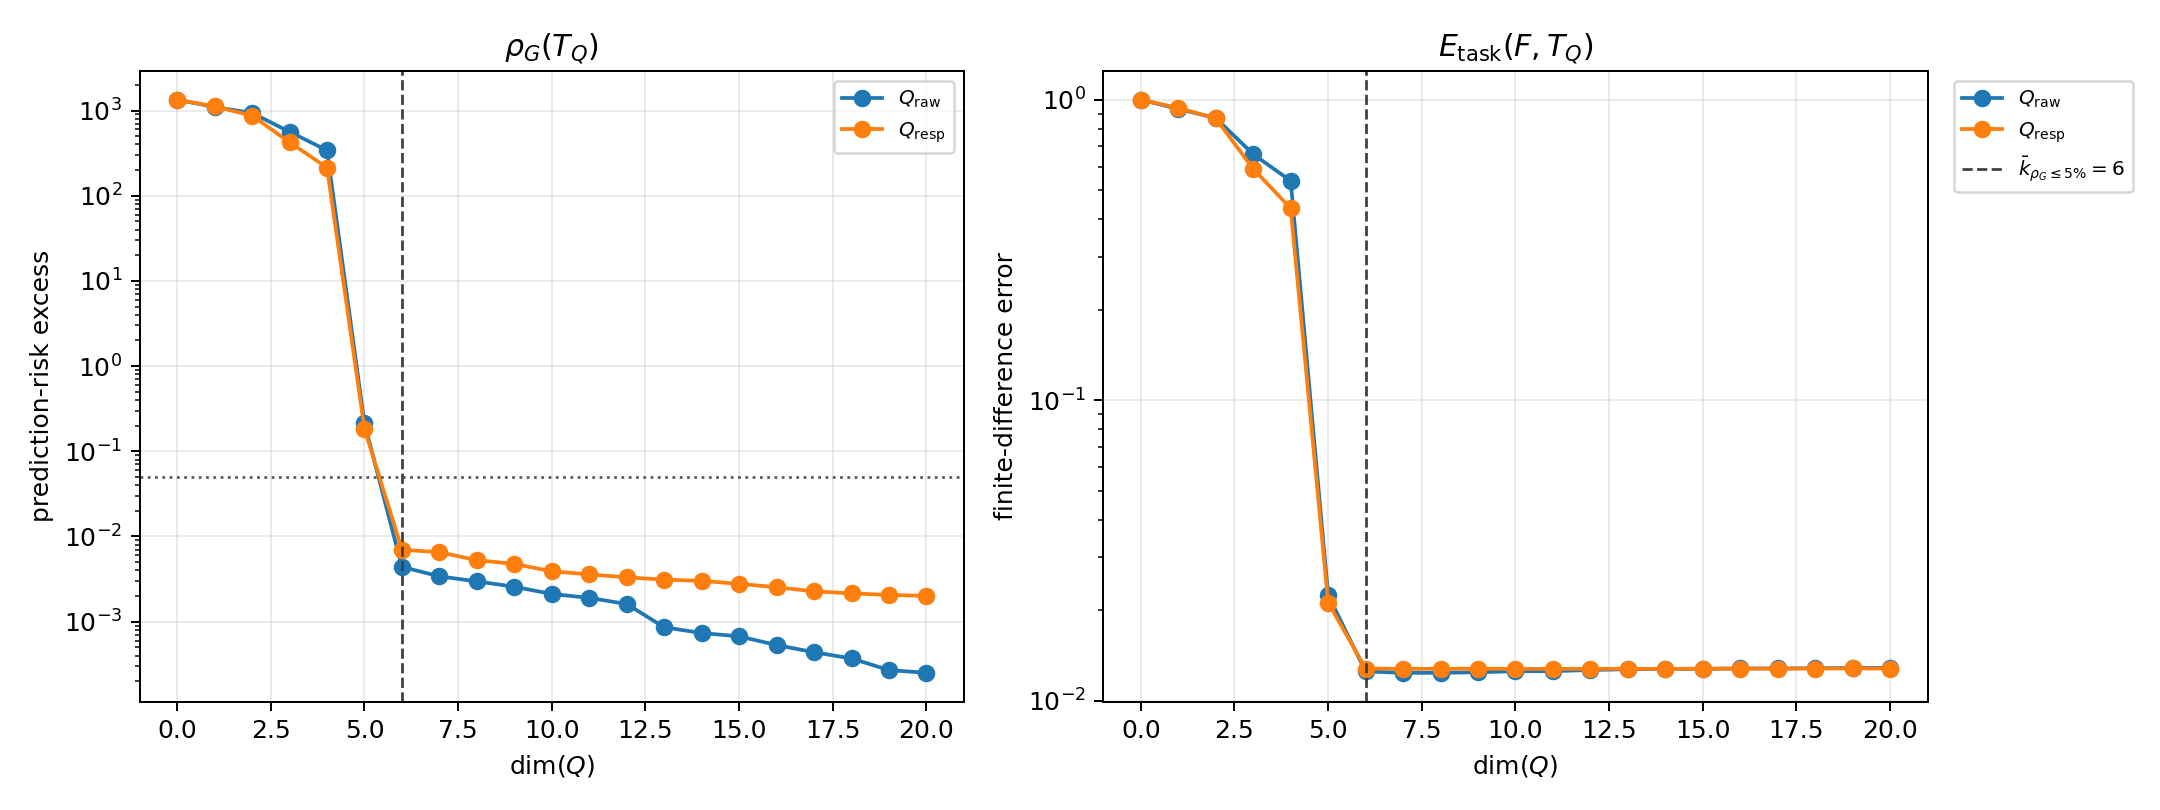
\includegraphics[width=0.92\linewidth]{../experiments/experiment_1_operator_certificate/results_more_probes_eps_sweep/eps_3e-3/rank_curves.png}
\caption{Experiment 1 rank-prefix curves. Left: \(\rho_G(T_Q)\), with the five-percent tolerance.
Right: \(E_{\mathrm{task}}(F,T_Q)\). The dashed line marks \(k_{\rho\le5\%}=6\).}
\label{fig:exp1-rank-curves}
\end{figure}

\begin{figure}[htbp]
\centering
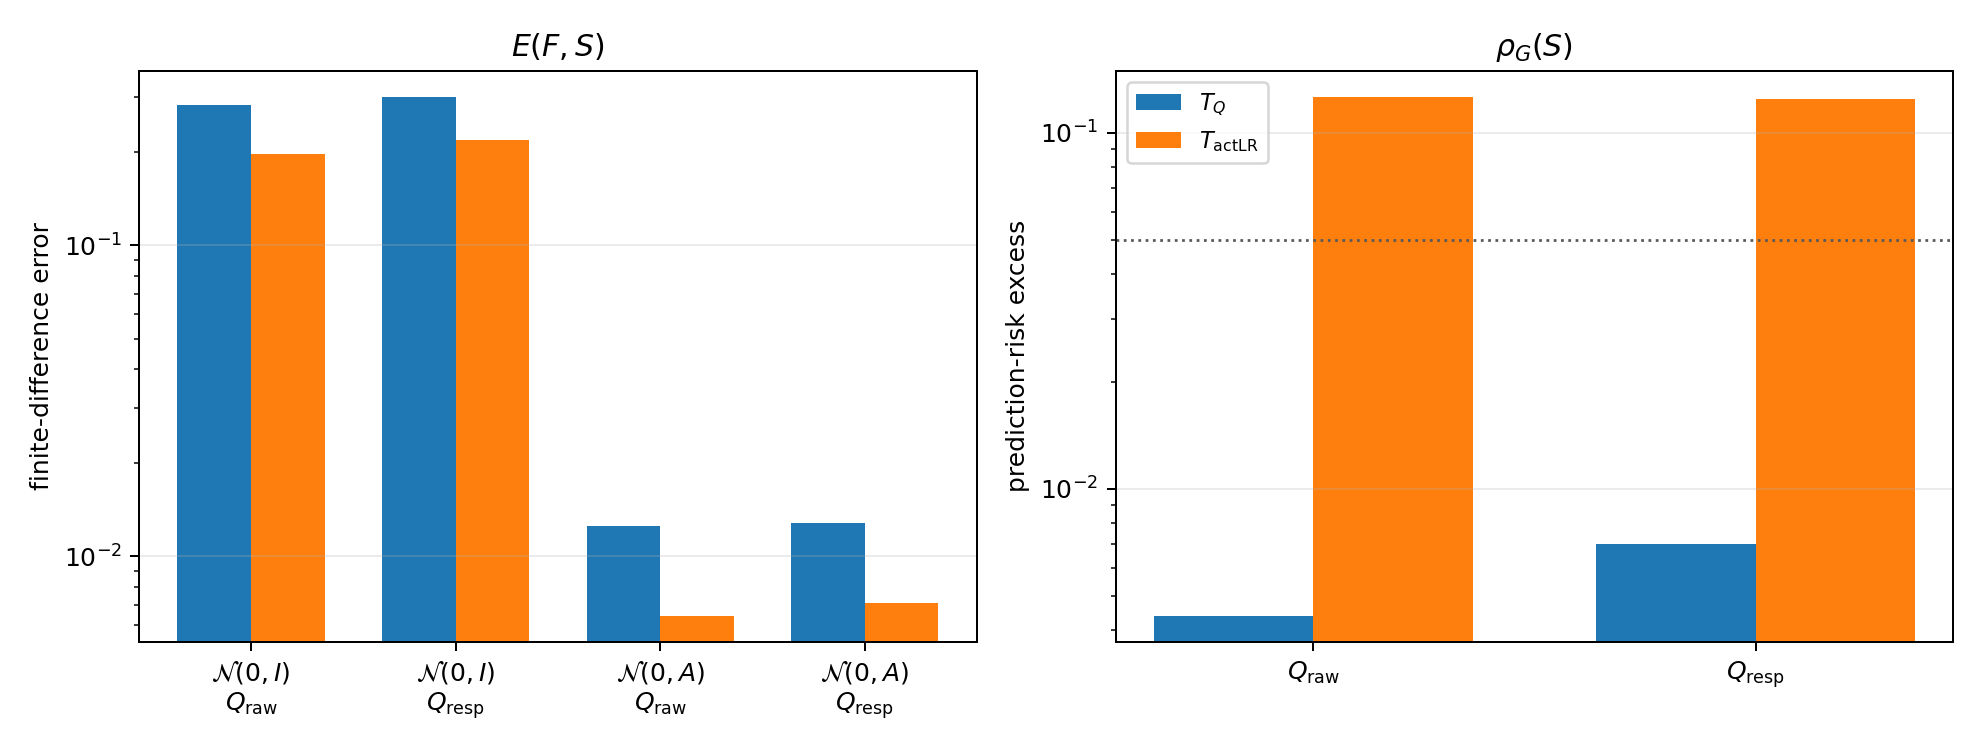
\includegraphics[width=0.90\linewidth]{../experiments/experiment_1_operator_certificate/results_more_probes_eps_sweep/eps_3e-3/actlr_comparison.png}
\caption{Experiment 1 same-span readout control. actLR uses the same activation coordinates
\(Q^\top u\) but fits a free least-squares readout; \(T_Q\) uses the KRR-constrained readout
\(K_tQ\).}
\label{fig:exp1-actlr-control}
\end{figure}

For probe-law interpolation,
\[
u_\lambda=\sqrt{1-\lambda}\,u_{\mathrm{task}}+\sqrt{\lambda}\,u_{\mathrm{iso}},
\qquad
\lambda\in[0,1],
\]
where \(u_{\mathrm{task}}\sim\mathcal{N}(0,A)\) and \(u_{\mathrm{iso}}\sim\mathcal{N}(0,I)\).
\(\lambda=0\) is task-label probing; \(\lambda=1\) is isotropic probing. A fresh matched response
basis \(Q_\lambda\) is built for each \(\lambda\).

\begin{figure}[htbp]
\centering
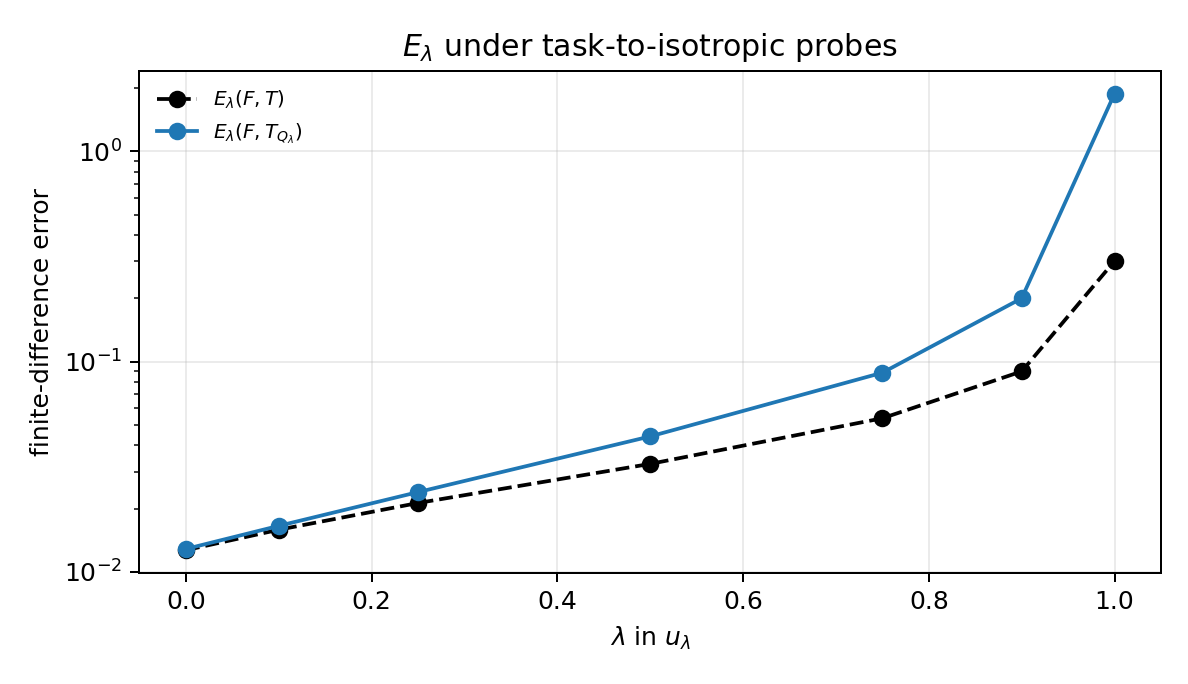
\includegraphics[width=0.70\linewidth]{../experiments/experiment_1_operator_certificate/results_more_probes_eps_sweep/eps_3e-3/probe_interpolation.png}
\caption{Experiment 1 task-to-isotropic interpolation. KRR-like local behavior degrades as
perturbations leave the task-distributed directions.}
\label{fig:exp1-probe-interpolation}
\end{figure}

At \(\varepsilon=3\cdot10^{-3}\), the normalized additivity defect is
\[
1.41\times10^{-4}
\]
on task probes and
\[
1.79\times10^{-3}
\]
on isotropic probes. Thus the finite-difference operator comparison is locally meaningful.

The epsilon sweep checks that this is not a fragile finite-difference scale choice:
\[
\begin{array}{ccccc}
\varepsilon
& E_{\mathrm{task}}(F,T)
& E_{\mathrm{task}}(F,T_{Q,\mathrm{raw}})
& E_{\mathrm{task}}(F,T_{Q,\mathrm{resp}})
& A_\varepsilon(F)\text{ task}\\
\hline
3\cdot10^{-3} & 0.01284 & 0.01252 & 0.01279 & 1.41\cdot10^{-4}\\
10^{-2} & 0.01284 & 0.01252 & 0.01280 & 2.77\cdot10^{-4}\\
3\cdot10^{-2} & 0.01284 & 0.01252 & 0.01279 & 8.13\cdot10^{-4}\\
10^{-1} & 0.01284 & 0.01251 & 0.01279 & 2.57\cdot10^{-3}\\
3\cdot10^{-1} & 0.01276 & 0.01243 & 0.01269 & 6.55\cdot10^{-3}\\
10^0 & 0.01237 & 0.01207 & 0.01230 & 1.43\cdot10^{-2}
\end{array}
\]
The operator estimate is stable through \(3\cdot10^{-1}\) and still reasonable at \(10^0\). The
additivity defect is smallest near \(3\cdot10^{-3}\) and rises at \(10^{-1}\)--\(10^0\), so
\(\varepsilon=3\cdot10^{-3}\)--\(10^{-2}\) is the clean finite-difference window for the certificate.

\FloatBarrier

\section{Experiment 2: Prediction-Risk Rank and Layerwise Availability}

Experiment 2 separates the intrinsic KRR rank from representation-dependent availability. The
intrinsic rank \(r_T\) is computed from
\[
C_G=K_tA^{-1/2}
\]
before seeing activations. The layerwise rank \(k_\ell^{5\%}\) asks how many directions from the
response span \(C_\ell=\spanop(D_yH_\ell^{\mathrm{ctx}})\) are needed for
\[
\rho_G\le0.05.
\]
Prefixes are evaluated by
\[
\rho_G(T_{Q_{\ell,k}})
=
\frac{\|(T-T_{Q_{\ell,k}})A^{1/2}\|_F^2}{R_{\mathrm{KRR}}+\eta_{\mathrm{num}}}.
\]
In tables, ``cand. dim.'' is \(\dim C_\ell\), ``rank to 5\%'' is \(k_\ell^{5\%}\), ``best
excess'' is \(\min_k\rho_G(T_{Q_{\ell,k}})\), and ``reach'' is the fraction of episodes where some
prefix reaches the five-percent target.

All Experiment 2 runs use \(\varepsilon=10^{-3}\), \(\alpha=0.05\), \(\sigma^2=0.1\),
16 build task probes, 16 held-out task probes, 8 layers, \(D=128\), 4 heads, and candidate basis
kinds response/raw/combined; the main tables report the response basis unless stated otherwise.
There is no artificial rank cap in the reported diagnostics: after numerical SVD cleanup by
\(\tau_{\mathrm{sv}}\), every prefix \(k=0,\ldots,\dim C_\ell\) is evaluated.
For each episode,
\[
A=K+\sigma^2 I,\qquad T=K_tA^{-1}.
\]
The flat linear family uses
\[
c\sim\mathrm{Unif}[1,10],
\qquad
x_i\sim\mathcal{N}(0,cI_{d_x}),
\qquad
\beta\sim\mathcal{N}(0,I_{d_x}),
\]
\[
y_i^{\mathrm{ctx}}=x_i^{\mathrm{ctx}\top}\beta+\epsilon_i,
\qquad
\epsilon_i\sim\mathcal{N}(0,\sigma^2),
\qquad
y_i^{\mathrm{tgt}}=x_i^{\mathrm{tgt}\top}\beta,
\]
and evaluates with the linear kernel
\[
K=X_{\mathrm{ctx}}X_{\mathrm{ctx}}^\top,
\qquad
K_t=X_{\mathrm{tgt}}X_{\mathrm{ctx}}^\top,
\qquad
K_{tt}=X_{\mathrm{tgt}}X_{\mathrm{tgt}}^\top .
\]
The \(d_x=40\) checkpoint keeps the same linear evaluation kernel but samples a random covariance
\(\Sigma=U\operatorname{diag}(\lambda)U^\top\), then
\[
x_i\sim\mathcal{N}(0,\Sigma),
\qquad
\tau(\Sigma)=\sum_{j=1}^{40}\frac{\lambda_j}{\lambda_j+\sigma^2}\le16.
\]
The native training window is
\[
\log_{10}\lambda_1\in[-2,2],
\qquad
n_{\mathrm{tgt}}=8,\qquad
n_{\mathrm{ctx}}=\operatorname{round}(\gamma\tau(\Sigma)),
\qquad
\gamma\in\{4,8,12\}.
\]
The spectrum is either a smooth log-decay or a step spectrum, with \(\tau(\Sigma)\) sampled in the
feasible part of \([10^{-3},16]\). The \(d_x=40\) diagnostic below reconstructs the native
validation bank: 30 batches of size 16, seed \(122\), with each batch sharing one sampled spectrum
and one \(\gamma\). The RBF family uses
\[
x_i\sim\mathcal{N}(0,I_5),
\qquad
\kappa(x,x')=\exp\!\left(-\frac{\|x-x'\|_2^2}{2\ell^2}\right),
\qquad
\ell=3.0,
\]
signal variance \(1.0\), and latent draw
\[
f\mid X\sim\mathcal{N}(0,K_{\mathrm{full}}+10^{-5}I),
\qquad
y^{\mathrm{ctx}}=f_{\mathrm{ctx}}+\epsilon,
\qquad
\epsilon\sim\mathcal{N}(0,\sigma^2I),
\qquad
y^{\mathrm{tgt}}=f_{\mathrm{tgt}}.
\]
For RBF evaluation, \(K,K_t,K_{tt}\) are the finite matrices induced by the same \(\kappa\). Episode
counts differ by run:
\[
\begin{array}{lccc}
\text{run} & \text{episodes} & n_{\mathrm{ctx}} & n_{\mathrm{tgt}}\\
\hline
\text{small linear }d_x\in\{3,5,8,10,15\} & 16\text{ each} & 47 & 16\\
\text{main RBF }128\times128 & 8 & 128 & 128\\
d_x=40\text{ native validation bank} & 480 & 3\text{--}187 & 8\\
\text{older fixed-}\ell=3\text{ RBF }n_{\mathrm{tgt}}\in\{16,64,128\} & 16\text{ each} & 47 & n_{\mathrm{tgt}}
\end{array}
\]
Seeds are \(42\) except for the \(d_x=40\) runs, which use seed \(122\). The RBF runs use
lengthscale \(3.0\) and signal variance \(1.0\). The main RBF run uses
\(\tau_{\mathrm{sv}}=10^{-4}\); the other Experiment 2 runs use \(\tau_{\mathrm{sv}}=10^{-3}\).

The linear sweep uses
\path{linear_sweep_dx3.pt}, \path{linear_sweep_dx5.pt}, \path{linear_sweep_dx8.pt},
\path{linear_sweep_dx10.pt}, and \path{linear_sweep_dx15.pt}. All are 8-layer, \(D=128\), 4-head
linear checkpoints. For \(d_x=3,5,8,10,15\), with
\[
n_{\mathrm{ctx}}=47,\qquad n_{\mathrm{tgt}}=16,
\]
the diagnostic recovers \(r_T\approx d_x\) up to the target cap.

\begin{table}[htbp]
\centering
\caption{Experiment 2 linear calibration. ``First layer'' is the first layer whose response span
reaches \(\rho_G\le0.05\).}
\scriptsize
\setlength{\tabcolsep}{4pt}
\renewcommand{\arraystretch}{0.9}
\begin{tabular}{lrrrrr}
\toprule
Checkpoint & \(r_T\) & first layer & final cand. dim. & \(k_L^{5\%}\) & \(E_{\mathrm{task}}(F,T)\)\\
\midrule
\(d_x=3\)  & 3.0  & 0 & 27.5 & 3.0  & 0.00617\\
\(d_x=5\)  & 5.0  & 0 & 27.6 & 5.0  & 0.00918\\
\(d_x=8\)  & 8.0  & 0 & 40.1 & 8.0  & 0.01250\\
\(d_x=10\) & 10.0 & 0 & 40.4 & 10.0 & 0.01433\\
\(d_x=15\) & 14.9 & 2 & 46.6 & 14.9 & 0.01735\\
\bottomrule
\end{tabular}
\renewcommand{\arraystretch}{1}
\end{table}

The main emergence checkpoint is
\path{rbf_fixed_l3_nctx128_ntgt128_seed42.pt}, trained on a fixed RBF kernel with lengthscale
\(3.0\), \(d_x=5\), \(D=128\), 8 layers, 4 heads, and 8 evaluation episodes,
\[
n_{\mathrm{ctx}}=128,\qquad n_{\mathrm{tgt}}=128.
\]
The model response is locally close to KRR:
\[
E_{\mathrm{task}}(F,T)=0.0306.
\]
On these 8 diagnostic episodes,
\[
\frac{\mathrm{MSE}_{\mathrm{model}}}{\mathrm{MSE}_{\mathrm{KRR}}}=1.03
\]
as an average of per-episode ratios.
For this finite KRR problem,
\[
r_T\approx24.75.
\]

\begin{table}[htbp]
\centering
\caption{Experiment 2 main emergence result: selected layers of the RBF \(128\times128\) checkpoint.
Here \(r_T\approx24.75\).}
\scriptsize
\setlength{\tabcolsep}{4pt}
\renewcommand{\arraystretch}{0.9}
\begin{tabular}{rrrr}
\toprule
Layer & cand. dim. & rank to 5\% & \(\rho_G(T_{Q_{\ell,r_T}})\)\\
\midrule
0 & 16  & --   & 1.147\\
1 & 51  & 38.0 & 0.100\\
2 & 84  & 26.9 & 0.058\\
4 & 107 & 25.2 & 0.050\\
8 & 119 & 24.9 & 0.048\\
\bottomrule
\end{tabular}
\renewcommand{\arraystretch}{1}
\end{table}

Layer 0 is insufficient. By layer 2, a nearly task-rank subspace is visible; by layers 4 and 8,
\(k_\ell^{5\%}\) matches \(r_T\) within finite-sample noise.

\begin{figure}[htbp]
\centering
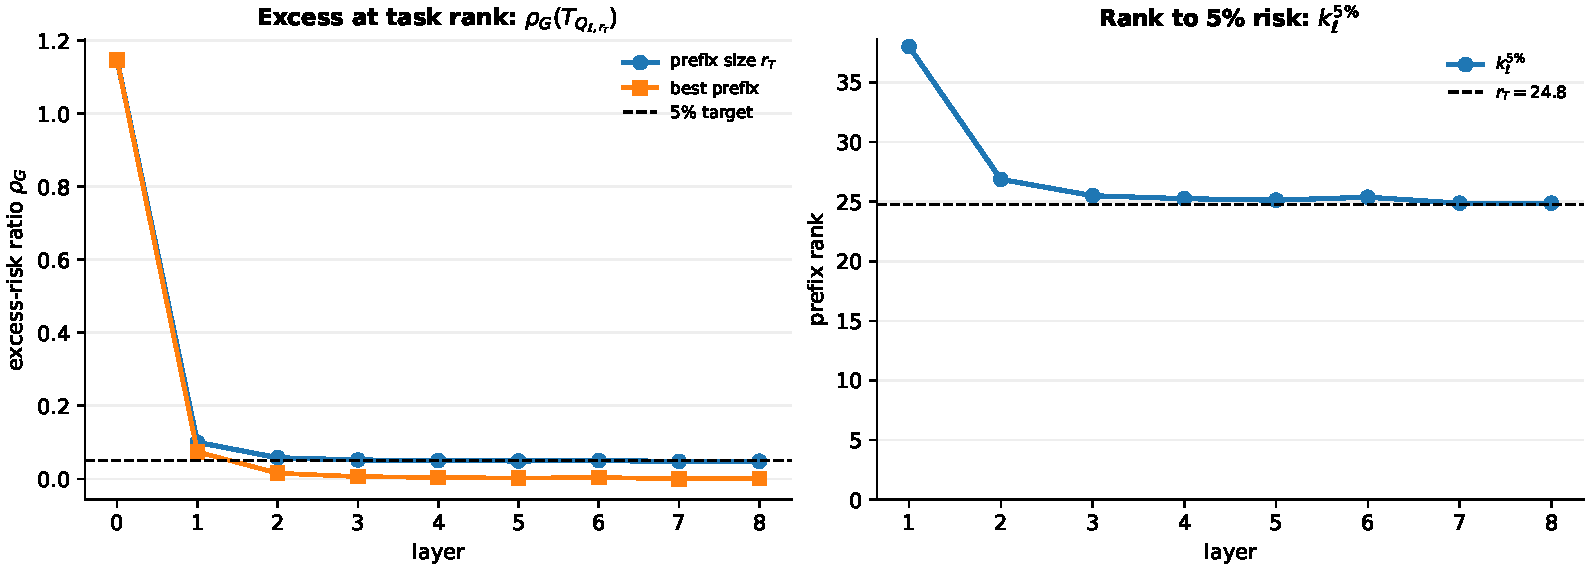
\includegraphics[width=0.95\linewidth]{../experiments/experiment_2_rank_emergence/results/rbf_128x128_seed42/emergence_response.pdf}
\caption{Experiment 2 layerwise emergence in the matched RBF \(128\times128\) checkpoint. Left:
\(\rho_G\) for the \(r_T\)-prefix and best prefix. Right: \(k_\ell^{5\%}\) against \(r_T\).}
\label{fig:exp2-rbf-emergence}
\end{figure}

\subsection{dx40 Native Bank: Scale-Stratified Availability and Removal}

The \(d_x=40\) checkpoint \path{dx40_tau16_s122.pt} is a scale-aware 8-layer, \(D=128\), 4-head
linear checkpoint trained with
\[
\begin{aligned}
n_{\mathrm{tgt}}&=8,
&
n_{\mathrm{ctx}}&=\operatorname{round}(\gamma\tau(\Sigma)),
&
\gamma&\in\{4,8,12\},\\
\log_{10}\lambda_1&\in[-2,2],
&
\tau(\Sigma)&=\sum_{i=1}^{40}\frac{\lambda_i}{\lambda_i+\sigma^2}\le16.
\end{aligned}
\]
The diagnostic uses the native validation bank:
\[
n_{\mathrm{tgt}}=8,\qquad
n_{\mathrm{ctx}}=\operatorname{round}(\gamma\tau(\Sigma)),
\qquad
480=30\times16\ \text{episodes}.
\]
Across these 480 episodes, \(n_{\mathrm{ctx}}\) ranges from \(3\) to \(187\). The average
pointwise ratio is
\[
\frac{\mathrm{MSE}_{\mathrm{model}}}{\mathrm{MSE}_{\mathrm{KRR}}}=1.638,
\]
as an average of per-episode ratios, with median \(1.236\) and aggregate means
\[
\mathrm{MSE}_{\mathrm{model}}=0.144,
\qquad
\mathrm{MSE}_{\mathrm{KRR}}=0.103.
\]

\begin{table}[htbp]
\centering
\caption{\(d_x=40\) native validation-bank response-span diagnostic, stratified by scale.
``Rank to \(5\%\)'' is averaged over reaching episodes.}
\scriptsize
\setlength{\tabcolsep}{4pt}
\renewcommand{\arraystretch}{0.9}
\begin{tabular}{@{}lrrrrr@{}}
\toprule
\(\log_{10}\lambda_1\) & \(n\) & reach & \(r_T\) & \(k_8^{5\%}\) &
\(\rho_G(T_{Q_{8,r_T}})\)\\
\midrule
\([-2,-1)\) & 112 & 1.000 & 6.42 & 6.42 & 0.0167\\
\([-1,0)\)  & 176 & 1.000 & 7.99 & 7.99 & 0.0005\\
\([0,1)\)   & 96  & 0.927 & 8.00 & 8.00 & 0.0171\\
\([1,2]\)   & 96  & 0.188 & 7.04 & 3.11 & 0.2232\\
\bottomrule
\end{tabular}
\renewcommand{\arraystretch}{1}
\end{table}

The full-bank average says the response basis usually appears:
\[
\mathbb{E}[r_T]=7.44,
\qquad
\mathbb{E}[k_8^{5\%}\mid \text{reach}]=7.33,
\qquad
\Pr(\text{reach at layer }8)=395/480=0.823.
\]
The scale-stratified result is sharper. For
\(\log_{10}\lambda_1<1\), the final response span almost always contains a KRR-sufficient prefix.
For \(\log_{10}\lambda_1\in[1,2]\), the certificate usually fails: only \(18/96\) episodes reach
\(\rho_G\le0.05\). Thus the dx40 model generally forms the relevant basis at low and moderate
scale, but high-scale episodes are a distinct failure mode.

\begin{figure}[htbp]
\centering
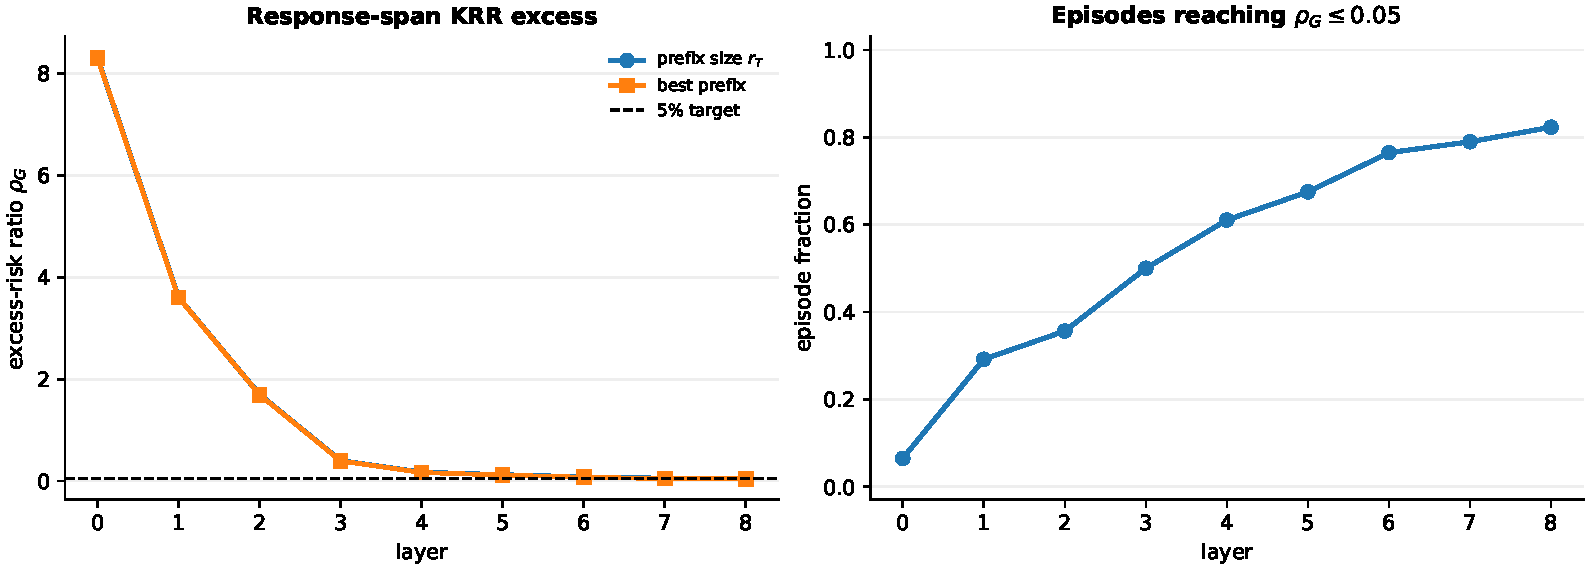
\includegraphics[width=0.95\linewidth]{../experiments/experiment_2_rank_emergence/results/dx40_validation_bank_full/emergence_response_reach.pdf}
\caption{Experiment 2 \(d_x=40\) native validation-bank diagnostic. With all retained prefixes
evaluated, the response span increasingly reaches the five-percent target across layers and succeeds
on \(82.3\%\) of episodes by the final layer.}
\label{fig:exp2-dx40-native}
\end{figure}

To test use, apply the same final response-prefix intervention as in Experiment 3: extract \(Q\)
from the final layer, but intervene at residual state \(s=1\), i.e. after the first transformer
block and before the second. Report one row per scale bin; the certificate information is carried
by \(\rho_G(T_Q)\), rather than by splitting a scale bin into separate certified and non-certified
rows. The summary below uses medians.

\begin{table}[htbp]
\centering
\caption{\(d_x=40\) native-bank intervention check by scale. Entries are medians over episodes in
the scale bin. Here \(k=\dim Q\) is the selected final-layer response-prefix size, and the MSE
columns are MSE/KRR ratios after no surgery, keep-\(Q\), and remove-\(Q\) at residual state \(s=1\).}
\scriptsize
\setlength{\tabcolsep}{4pt}
\renewcommand{\arraystretch}{0.9}
\begin{tabular}{@{}lrrrrrr@{}}
\toprule
\(\log_{10}\lambda_1\) & \(r_T\) & \(k\) & \(\rho_G(T_Q)\) &
base MSE/KRR & keep-\(Q\) MSE/KRR & remove-\(Q\) MSE/KRR\\
\midrule
\([-2,-1)\) & 7 & 7  & \(1.32\cdot10^{-2}\) & 1.07 & 1.31 & 2.12\\
\([-1,0)\)  & 8 & 8  & \(2.18\cdot10^{-26}\) & 1.16 & \(1.10\cdot10^5\) & \(8.71\cdot10^3\)\\
\([0,1)\)   & 8 & 8  & \(3.56\cdot10^{-4}\) & 1.53 & \(5.36\cdot10^{14}\) & \(4.22\cdot10^{14}\)\\
\([1,2]\)   & 8 & 19 & 0.194 & 2.13 & \(1.29\cdot10^{15}\) & \(7.19\cdot10^{14}\)\\
\bottomrule
\end{tabular}
\renewcommand{\arraystretch}{1}
\end{table}

The projection algebra is the intended \(A\)-orthogonal intervention:
\[
\text{keep }Q:\ H_s^{\mathrm{ctx}}\mapsto QQ^\top A H_s^{\mathrm{ctx}},
\qquad
\text{remove }Q:\ H_s^{\mathrm{ctx}}\mapsto H_s^{\mathrm{ctx}}-QQ^\top A H_s^{\mathrm{ctx}}.
\]
The strange numbers are therefore not from the certified/non-certified split. They show that this
early-state residual surgery is dynamically unstable on much of the native bank: even when
\(\rho_G(T_Q)\) certifies that the induced operator is KRR-sufficient, replacing the actual state by
its \(Q\)-projection can move the residual stream far off the transformer's typical trajectory.
Thus this native-bank table is an instability diagnostic, not the clean repair experiment.

For the older fixed-\(\ell=3\) RBF checkpoint, the final-layer response diagnostic at
\(n_{\mathrm{ctx}}=47\) is:

\begin{table}[htbp]
\centering
\caption{Older fixed-\(\ell=3\) RBF checkpoint, final-layer response diagnostic.}
\label{tab:exp2-old-rbf}
\begin{tabular}{ccccc}
\toprule
\(n_{\mathrm{tgt}}\) & \(r_T\) & \(k_L^{5\%}\) & \(\rho_G(T_{Q_{L,r_T}})\) & \(E_{\mathrm{task}}(F,T)\)\\
\midrule
16  & 10.6 & 11.1 & 0.049 & 0.067\\
64  & 17.1 & 17.8 & 0.053 & 0.074\\
128 & 18.3 & 19.3 & 0.057 & 0.097\\
\bottomrule
\end{tabular}
\end{table}

Availability can remain near-sufficient while the realized finite-difference operator becomes less
clean.

\section{Experiment 3: Causal Direction Removal}

Experiments 1--2 show availability. Experiment 3 tests use: take a certified raw final basis
\[
Q=[q_1,\ldots,q_r],
\]
rank its directions by KRR task leverage, remove selected context-token residual directions, and
roll the remaining layers forward.

The checkpoint is \path{linear_baseline_dx5_L8.pt}. The diagnostic uses flat-spectrum linear
episodes with
\[
d_x=5,\qquad
n_{\mathrm{ctx}}=47,\qquad
n_{\mathrm{tgt}}=16,\qquad
\sigma^2=0.1,
\]
\[
\varepsilon=10^{-3},
\]
32 episodes, seed \(42\), 32 held-out causal probes per episode, \(\tau_{\mathrm{sv}}=10^{-3}\),
\(r_{\max}=12\), task and isotropic probes, residual-state sweep \(s=0,\ldots,8\), and
\(k_{\mathrm{remove}}\in\{1,2,4\}\). The complement-ablation summary uses 8 episode records per
condition.

For \(Q_{-j}\), the basis with \(q_j\) removed, define task leverage
\[
\Lambda_j^{\mathrm{red}}(U)
:=
\left(
\frac{
\sum_{u\in U}\|(T_Q-T_{Q_{-j}})u\|_2^2
}{
\sum_{u\in U}\|Tu\|_2^2+\eta_{\mathrm{num}}
}
\right)^{1/2}.
\]
High-leverage directions are those whose removal most changes the reduced KRR response. For a
selected \(A\)-orthonormal block \(D=Q_J\), define the context-side \(A\)-projection
\[
P_D^A:=DD^\top A,
\qquad
D^\top A D=I.
\]
Direction-removal surgery at residual state \(s\) changes only context-token residuals:
\[
H_s^{\mathrm{ctx}}
\longmapsto
(I-P_D^A)H_s^{\mathrm{ctx}}.
\]
Target-token residuals are left unchanged, and the transformer is rolled forward from state \(s\).
For the whole-subspace complement ablation, use \(D=Q\):
\[
\text{keep }Q:\quad
H_s^{\mathrm{ctx}}\mapsto P_Q^A H_s^{\mathrm{ctx}}=QQ^\top A H_s^{\mathrm{ctx}},
\]
\[
\text{remove }Q:\quad
H_s^{\mathrm{ctx}}\mapsto (I-P_Q^A)H_s^{\mathrm{ctx}}
=H_s^{\mathrm{ctx}}-QQ^\top A H_s^{\mathrm{ctx}}.
\]
Matched controls remove low-task-leverage directions, high-isotropic-but-low-task directions,
high-activation-variance-but-low-task directions, and random subsets.

Prediction drift is
\[
\|F_{\mathrm{surg}}(y)-F_{\mathrm{base}}(y)\|/\|F_{\mathrm{base}}(y)\|.
\]
KRR-error inflation is post-surgery pointwise KRR error divided by pre-surgery pointwise KRR error.
Response damage is
\[
\left(
\frac{\sum_{u\in U}\|D_\varepsilon F_{\mathrm{surg}}(y)[u]
-D_\varepsilon F_{\mathrm{base}}(y)[u]\|_2^2}
{\sum_{u\in U}\|Tu\|_2^2+\eta_{\mathrm{num}}}
\right)^{1/2}.
\]

Before surgery,
\[
E_{\mathrm{task}}(F,T)=0.00926,
\qquad
E_{\mathrm{task}}(F,T_Q)=0.00920,
\qquad
\rho_G(T_Q)=0.00149.
\]
Off task,
\[
E_{\mathrm{iso}}(F,T)=0.266.
\]

\begin{table}[htbp]
\centering
\caption{Experiment 3 causal-use summary. Direction removals are at residual state \(s=1\).}
\small
\setlength{\tabcolsep}{4pt}
\begin{tabular}{@{}p{0.32\linewidth}p{0.30\linewidth}p{0.30\linewidth}@{}}
\toprule
Intervention & Result & Reading\\
\midrule
No surgery &
\(E_{\mathrm{task}}(F,T)=0.00926\), \(\rho_G(T_Q)=0.00149\) &
Starting episodes satisfy the task-local certificate.\\
Remove one high-task-leverage direction &
prediction drift \(4.68\), response damage \(41.59\), KRR-error inflation \(649\times\) &
KRR-leverage directions are causally important.\\
Remove one low-task-leverage direction &
prediction drift \(9.8\times10^{-4}\), response damage \(0.0024\), inflation \(1.03\times\) &
Low-task-leverage same-basis removals are nearly inert.\\
Keep only the \(Q\)-projection &
\(E_{\mathrm{task}}(F,T)=0.01836\), response damage \(0.01634\) &
The certified subspace nearly preserves the task-local response.\\
Remove \(Q\) &
\(E_{\mathrm{task}}(F,T)=106.46\), response damage \(106.46\) &
The complement does not carry the task-local KRR response.\\
\bottomrule
\end{tabular}
\end{table}

For the \(d_x=40\) target-rich run, the causal check is repeated on the Experiment 2 response
prefix rather than on a raw final basis. For each episode, build the final-layer response candidate
span \(C_8=\spanop(D_yH_8^{\mathrm{ctx}})\), order it by KRR-targeted energy, and choose
\[
k=\min\{j:\rho_G(T_{Q_{8,j}})\le0.05\}.
\]
Then apply the same complement ablation at residual state \(s=1\). This tests the actual
near-minimal response prefix, not the whole \(47\)-dimensional candidate span.

\begin{table}[htbp]
\centering
\caption{\(d_x=40\) causal-use check on the final-layer response prefix. Eight episodes, seed
\(122\), \(n_{\mathrm{ctx}}=47\), \(n_{\mathrm{tgt}}=40\), 16 build probes, 16 held-out task probes,
\(\varepsilon=10^{-3}\).}
\small
\setlength{\tabcolsep}{4pt}
\begin{tabular}{@{}lcccccc@{}}
\toprule
Intervention & rank \(Q\) & \(r_T\) & \(\rho_G(T_Q)\) & drift & \(E_{\mathrm{task}}(F,T)\) & damage\\
\midrule
No surgery & \(21.38\) & \(21.00\) & \(0.0410\) & \(0\) & \(0.0988\) & \(0\)\\
Keep \(Q\) & \(21.38\) & \(21.00\) & \(0.0410\) & \(0.154\) & \(0.156\) & \(0.156\)\\
Remove \(Q\) & \(21.38\) & \(21.00\) & \(0.0410\) & \(0.640\) & \(0.592\) & \(0.581\)\\
\bottomrule
\end{tabular}
\end{table}

Thus the dx40 model does use the KRR-sufficient response prefix: deleting it is much more damaging
than keeping it. The mediation is weaker than in the \(d_x=5\) certificate, since keep-\(Q\) is not
nearly identical to the base model, but the effect is selective and in the expected direction.

High-task surgery is most damaging at early residual states. At \(s=1\), aggregate task leverage and
task response damage are strongly related across matched non-random controls:
\[
\text{log--log Pearson }0.91,
\qquad
\text{Spearman }0.87.
\]

\begin{figure}[htbp]
\centering
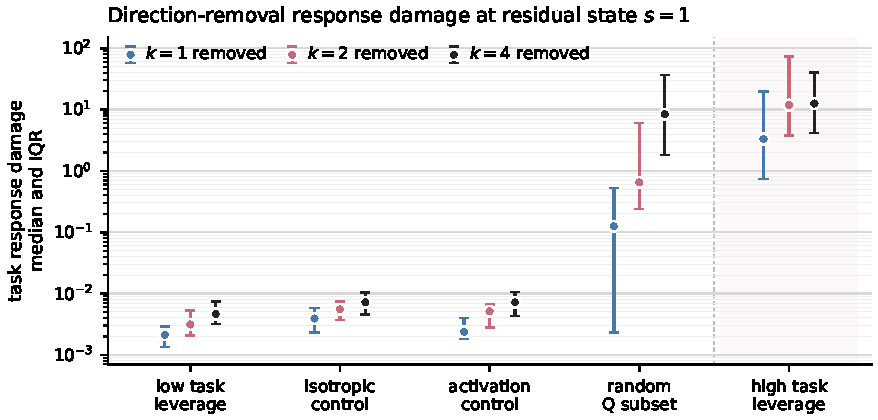
\includegraphics[width=0.78\linewidth]{../experiments/experiment_3_causal_surgery/results/experiment_3_key_surgery.pdf}
\caption{Experiment 3 selective causal effect. High task-leverage removals cause much larger task
finite-difference response damage than matched low-task-leverage controls.}
\end{figure}

\begin{figure}[htbp]
\centering
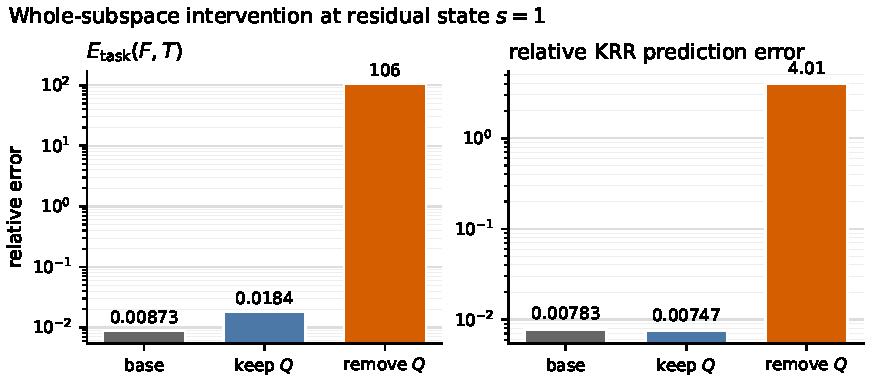
\includegraphics[width=0.82\linewidth]{../experiments/experiment_3_causal_surgery/results_complement_ablation/complement_ablation_bars.pdf}
\caption{Experiment 3 whole-subspace complement ablation at \(s=1\). Left: task finite-difference
operator error \(E_{\mathrm{task}}(F,T)\) after no surgery, keep-\(Q\), and remove-\(Q\). Right:
relative pointwise KRR prediction error for the same three interventions. Keeping only
\(P_Q^AH_s^{\mathrm{ctx}}\) nearly preserves the task-local behavior; deleting it leaves the
complement and destroys the KRR response.}
\end{figure}

\FloatBarrier

\section{Experiment 4: Repair After Basis Formation}

Experiment 4 is a conditional repair test. First choose a setting where the model usually builds a
KRR-sufficient response basis. Then look only at the rare episodes where the model output is bad.
Finally test whether keeping the certified basis \(Q\) repairs those bad outputs.

Use the \(d_x=40\) checkpoint \path{dx40_tau16_s122.pt} in the target-rich diagnostic setting
\[
n_{\mathrm{ctx}}=47,
\qquad
n_{\mathrm{tgt}}=40,
\qquad
\log_{10}\lambda_1\in[-2,1].
\]
This is not the native validation distribution. It is a controlled setting in which the response
prefix usually exists, so a keep-\(Q\) repair has a chance to be principled.

For each episode, form the final-layer response candidate span
\[
C_8=\spanop(D_yH_8^{\mathrm{ctx}}),
\]
order it by KRR-targeted energy, and choose the first prefix satisfying
\[
Q=Q_{8,k},
\qquad
k=\min\{j:\rho_G(T_{Q_{8,j}})\le0.05\}.
\]
If no such prefix exists, record the episode as not certified.

Sample a 200-episode bank with seed \(20260506\). Before conditioning on outliers, the bank has the
following distribution:
\[
\begin{array}{c|cccc}
\text{quantity} & \text{mean} & \text{median} & q_{25}\text{--}q_{75} & \text{tail / range}\\
\hline
\mathrm{MSE}_{\mathrm{model}}/\mathrm{MSE}_{\mathrm{KRR}}
& 84.96 & 1.14 & 1.03\text{--}1.37 & q_{90}=1.67,\ q_{99}=4.19,\ \max=1.67\cdot10^4\\
r_T & 23.29 & 25 & 19.75\text{--}28 & 1\text{--}32\\
k & 23.76 & 25 & 20\text{--}29 & 1\text{--}41\\
\rho_G(T_Q) & 0.0445 & 0.0441 & 0.0400\text{--}0.0470 & \Pr(\rho_G(T_Q)\le0.05)=196/200
\end{array}
\]
The aggregate MSEs are
\[
\mathbb{E}\,\mathrm{MSE}_{\mathrm{model}}=0.579,
\qquad
\mathbb{E}\,\mathrm{MSE}_{\mathrm{KRR}}=0.131.
\]
Thus the bank is mostly non-pathological and basis-present: the median MSE ratio is \(1.14\), the
certificate holds on \(98\%\) of episodes, and the typical KRR rank and extracted prefix size are
both around \(23\)--\(25\). The large arithmetic mean MSE ratio is caused by one catastrophic
outlier, bank id \(35\); removing only this largest outlier gives mean ratio \(1.28\).

After this bank-level scan, select episodes where the unmodified model is bad:
\[
\frac{\mathrm{MSE}_{\mathrm{model}}}{\mathrm{MSE}_{\mathrm{KRR}}}\ge5.
\]
Only two episodes pass. The interventions are applied at residual state \(s=1\):
\[
\begin{aligned}
\text{keep }Q:\quad
&H_s^{\mathrm{ctx}}\mapsto QQ^\top A H_s^{\mathrm{ctx}},\\
\text{remove }Q:\quad
&H_s^{\mathrm{ctx}}\mapsto H_s^{\mathrm{ctx}}-QQ^\top A H_s^{\mathrm{ctx}},\\
\text{keep random }R:\quad
&H_s^{\mathrm{ctx}}\mapsto RR^\top A H_s^{\mathrm{ctx}},
\qquad R^\top AR=I,\quad \dim R=\dim Q.
\end{aligned}
\]
The random controls test whether repair is specific to the learned KRR-targeted prefix, or whether
same-dimensional residual-stream denoising already explains much of the effect.

\begin{table}[htbp]
\centering
\caption{Experiment 4 conditional repair after certified basis formation. The bank has 200
target-rich episodes; two satisfy \(\mathrm{MSE}_{\mathrm{model}}/\mathrm{MSE}_{\mathrm{KRR}}\ge5\).
Rows report averages over the two selected episodes; the random-control row also averages 20
same-rank \(A\)-orthonormal subspaces per selected episode.}
\small
\setlength{\tabcolsep}{4pt}
\begin{tabular}{@{}lccc@{}}
\toprule
Intervention & MSE & MSE/KRR & Reading\\
\midrule
Base & \(41.80\) & \(8371.3\) & pathological output\\
Keep \(Q\) & \(7.41\cdot10^{-3}\) & \(1.096\) & near-KRR repair\\
Keep random \(A\)-subspace & \(8.36\cdot10^{-3}\) & \(1.252\) & same-rank control also repairs\\
Remove \(Q\) & \(100.14\) & \(20056.4\) & worsens the failure\\
\bottomrule
\end{tabular}
\end{table}

The two selected episodes are:
\[
\begin{array}{c|cccccc}
\text{bank id} & r_T & k & \rho_G(T_Q) & \mathrm{MSE}_{\mathrm{KRR}} & \mathrm{MSE}_{\mathrm{base}} &
\mathrm{MSE}_{\mathrm{keep}\ Q} \\
\hline
35 & 2 & 4 & 0.0469 & 0.004991 & 83.531 & 0.005864\\
184 & 1 & 1 & 0.0371 & 0.008793 & 0.06009 & 0.008949
\end{array}
\]

Both outliers have \(\rho_G(T_Q)\le0.05\). Thus the KRR-sufficient response basis is present before
the intervention, which explains why keeping \(Q\) can move the bad output back to KRR-level MSE;
removing \(Q\) makes the failure worse. But the random control prevents a stronger uniqueness
claim, since a random same-rank \(A\)-subspace also repairs these two episodes. The clean conclusion
is that the bad outputs contain harmful residual components outside a small task-relevant subspace;
the learned \(Q\) is one principled way to keep the useful part, but same-dimensional denoising
already explains much of the effect.

\FloatBarrier

\section{Logical Chain}

\begin{enumerate}[label=\arabic*.]
\item Freeze the episode geometry \(G=(X_{\mathrm{ctx}},X_{\mathrm{tgt}})\).
\item Under fixed \(G\), ridge regression becomes \(T=K_tA^{-1}\).
\item Treat the transformer as a label map \(F:\R^{n_{\mathrm{ctx}}}\to\R^{n_{\mathrm{tgt}}}\).
\item Estimate the local response \(D_\varepsilon F(y)[u]\).
\item Test behavior with \(E_\varepsilon(F,T)\) on task-label probes.
\item Compute \(r_T\) from \(C_G=K_tA^{-1/2}\) and \(R_{\mathrm{KRR}}\).
\item Extract activation-derived context-side candidate spans \(C_\ell\).
\item Order each candidate span by KRR-targeted energy and form prefixes \(Q_{\ell,k}\).
\item Construct \(T_Q=K_tQQ^\top\).
\item Test subspace sufficiency with \(\rho_G(T_Q)\).
\item Test model-subspace alignment with \(E_\varepsilon(F,T_Q)\).
\item In causal runs, remove high-leverage \(Q\)-directions and measure task-local response damage.
\end{enumerate}

Mechanism story: behavioral similarity, KRR-structured activation certificate, risk-rank
sufficiency, layerwise availability, and validated causal specificity.

\end{document}
